\chapter{Energy Efficient Ethernet em Clusters Hadoop MapReduce}

Neste capítulo são apresentados os resultados das simulações de \emph{clusters Hadoop 3.x MapReduce} utilizando a ferramenta NetSLS e o \emph{Energy Efficient Ethernet} em modo \emph{Fast Wake} e \emph{Deep Sleep}. Através destes dados mostramos que uma boa economia de energia pode ser obtida em conexões de até 40GbE, enquanto conexões acima de 100GbE possuem problemas de performance quando o EEE está habilitado no modo \emph{Deep Sleep}.

\section{Economia de Energia}

Esta seção contém os dados de economia de energia obtidos das simulações com topologia \emph{leaf-spine} e conexões de 1GbE e 10GbE; 1GbE e 25GbE; 10GbE e 100GbE; 10GbE e 400GbE; 25GbE e 400GbE; e, finalmente, 40GbE e 400GbE. O restante da metodologia empregada pode ser visualizada no Capítulo 3 de forma detalhada.

\begin{figure}[htp]
    \centering
    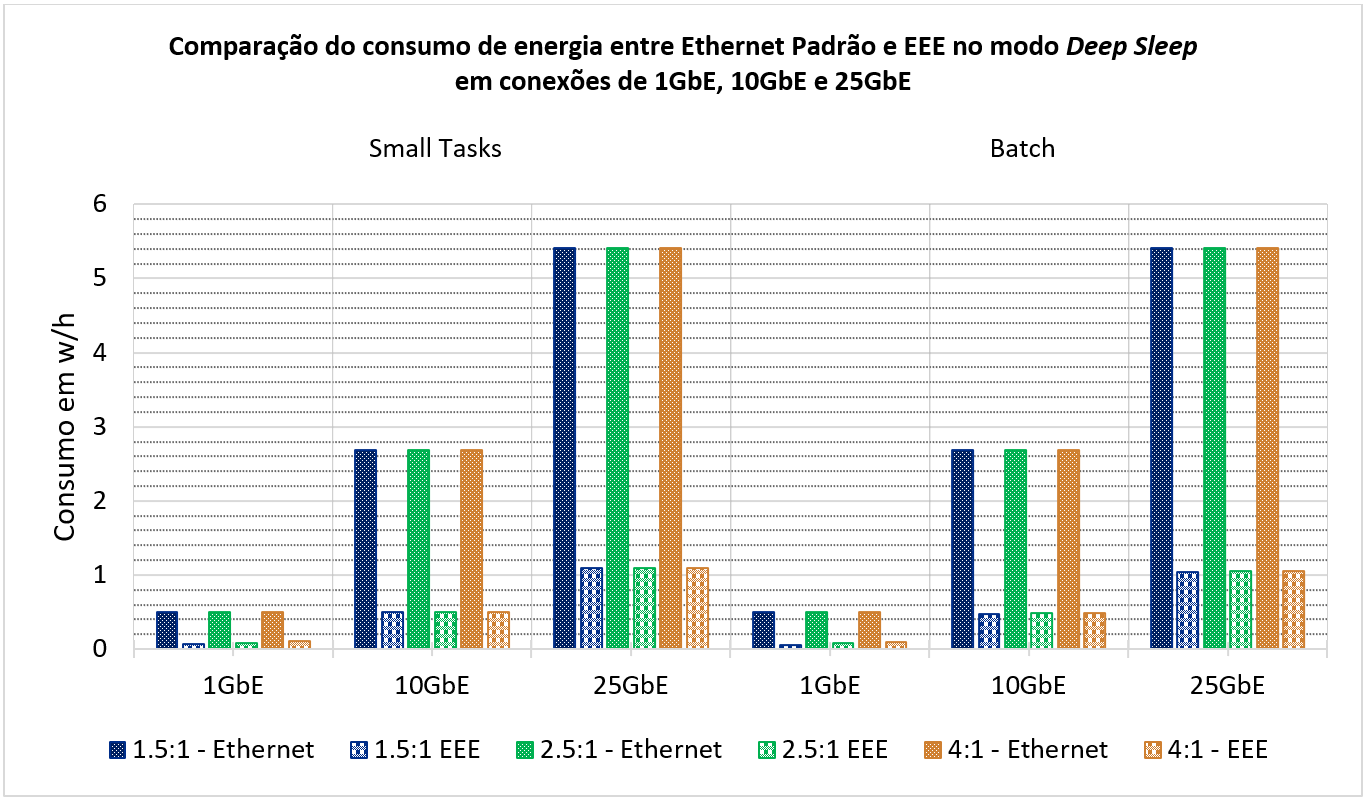
\includegraphics[width=16cm]{4-EEEHadoop/Image1_EEEConsumption1-10-25.PNG}
    \caption{\centering Comparação do consumo de energia entre \emph{Ethernet} Padrão e EEE no modo \emph{Deep Sleep} em conexões de 1GbE, 10GbE e 25GbE}
    \label{fig:EEEConsumption1-10-25}
\end{figure}

\begin{figure}[htp]
    \centering
    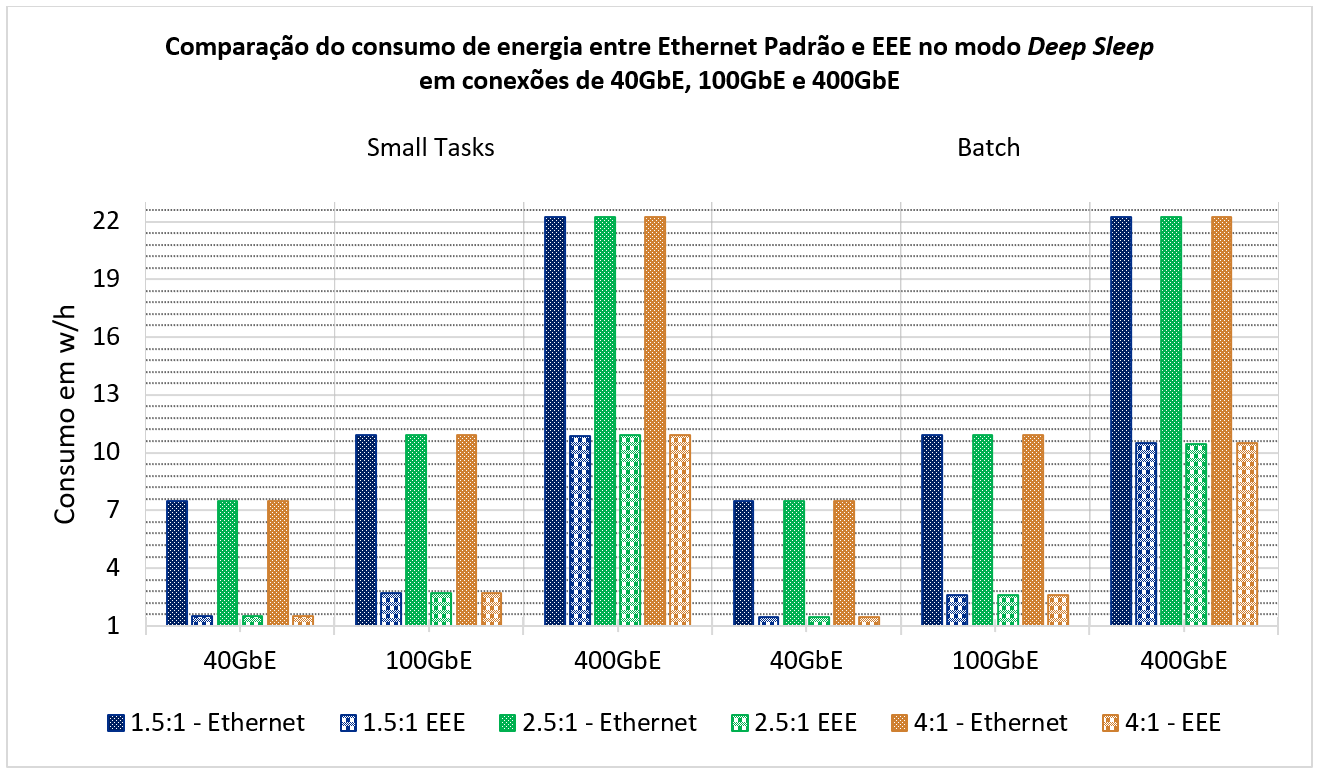
\includegraphics[width=16cm]{4-EEEHadoop/Image2_EEEConsumption40-100-400.PNG}
    \caption{\centering Comparação do consumo de energia entre \emph{Ethernet} Padrão e EEE no modo \emph{Deep Sleep} em conexões de 40GbE, 100GbE e 400GbE}
    \label{fig:EEEConsumption40-100-400}
\end{figure}

\begin{figure}[htp]
    \centering
    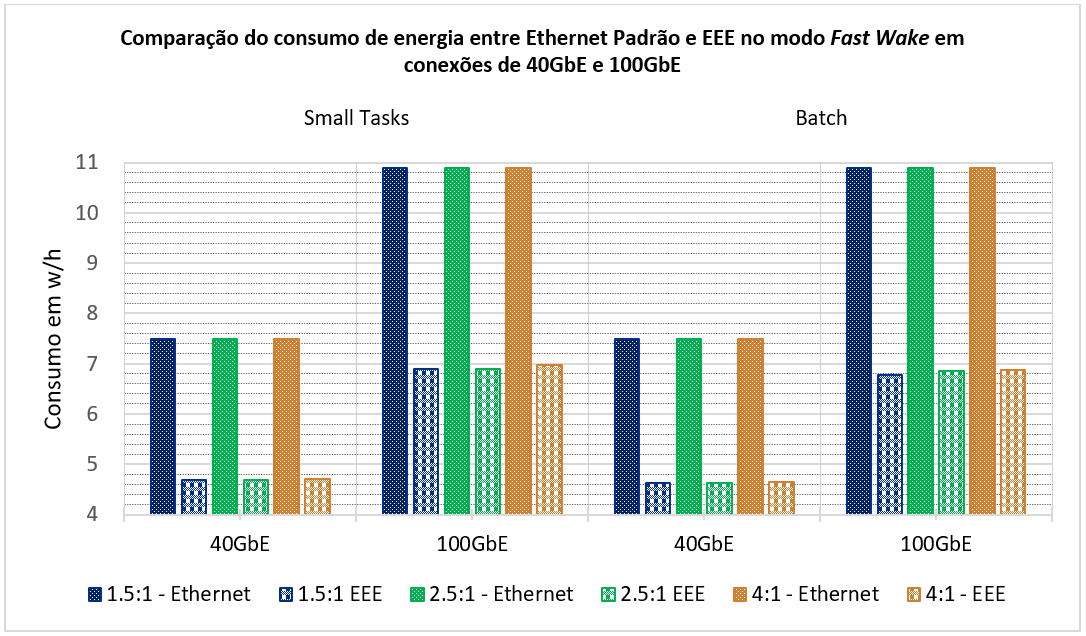
\includegraphics[width=16cm]{4-EEEHadoop/Image5_EEEConsumption40-100-FastWakeMode.PNG}
    \caption{\centering Comparação do consumo de energia entre \emph{Ethernet} Padrão e EEE no modo \emph{Fast Wake} em conexões de 40GbE e 100GbE}
    \label{fig:EEEConsumption100-400FastWakeMode}
\end{figure}

Através das simulações com o modo \textbf{\emph{Deep Sleep}} do EEE encontramos os dados mostrados nas figuras 4.1 e 4.2, que demonstram a economia de energia em \emph{Jobs MapReduce} em \emph{clusters}{} Hadoop 3.x, com reduções médias de 0,5w/h para 0,080w/h em links de 1GbE - redução de 83,89\%; 2,68w/h para 0,490w/h em 10GbE - redução de 81,68\%; de 5,41w/h para 1,072w/h em 25GbE - redução de 80,12\%; 7,49w/h para 1,487w/h em 40GbE - redução de 80,14\%; de 10,89w/h para 2,646w/h em 100GbE - redução de 75,69\%; e de 22,21w/h para 10,685w/h em 400GbE - redução de 51,89.

Usando a configuração de topologia de rede \emph{leaf-spine} recomendada pela Cisco, com uma taxa de assinatura excessiva igual a 4:1, encontramos resultados que, como em \cite{silva2018eon}; \cite{e2015exploring}; \cite{e2017energy}, apontam para economias de energia semelhantes habilitando o EEE no modo \textbf{\emph{Deep Sleep}} ao executar \emph{Small Tasks} e \emph{Batch Jobs}, no entanto, os \emph{Batch Jobs} tiveram um desempenho ligeiramente melhor.

Como pode-se observar na figura 4.3, ao habitarmos o EEE no modo \textbf{\emph{Fast Wake}} para as conexões de 40GbE e 100GbE, percebe-se uma economia de energia relativamente menor do que comparado ao modo \textbf{\emph{Deep Sleep}}, de 7,49w/h para 4,634w/h em conexões de 40GbE - redução de 38,13\%, e de 10,89w/h para 6,916w/h - redução de 36,49\% em conexões de 100GbE respectivamente. Em contrapartida, o desempenho foi melhor como detalhado na próxima seção.

\section{Desempenho}

Esta seção contém os dados de performance obtidos das simulações com topologia \emph{leaf-spine} e conexões de 1GbE e 10GbE; 1GbE e 25GbE; 10GbE e 100GbE; 10GbE e 400GbE; 25GbE e 400GbE; e, finalmente, 40GbE e 400GbE. O restante da metodologia empregada pode ser visualizada no Capítulo 3 de forma detalhada.

Ao contrário do que afirmam os fornecedores de equipamentos, nossos testes demonstram que é possível obter uma boa economia de energia habilitando o \emph{Energy Efficient Ethernet} no modo \textbf{\emph{Deep Sleep}}, com uma perda média de desempenho de praticamente zero para links de 1GbE - 0,21\%; 10GbE - 0,94\%; e 25GbE - 1,52\%; ou razoável no caso de 40GbE - 2,85\% conforme mostrado nas figuras 4.4 e 4.5. Para links de 100GbE e 400GbE há uma boa economia de energia, mas com uma perda de desempenho que não é considerada ideal, em torno de 4,55\% e 8,58\% respectivamente.

Em geral, ao habilitar o EEE em modo \textbf{\emph{Deep Sleep}} no \emph{cluster}, percebe-se que os \emph{Batch Jobs} obtêm melhor economia de energia e desempenho em relação aos \emph{Small Tasks}. Ainda é possível observar um cenário específico, em que ao diminuir a taxa de assinatura excessiva da rede para 1.5:1 em links 1GbE, os \emph{Batch Jobs} obtiveram uma melhora significativamente maior na economia de energia e no desempenho em comparação com outras conexões.

\begin{figure}[htp]
    \centering
    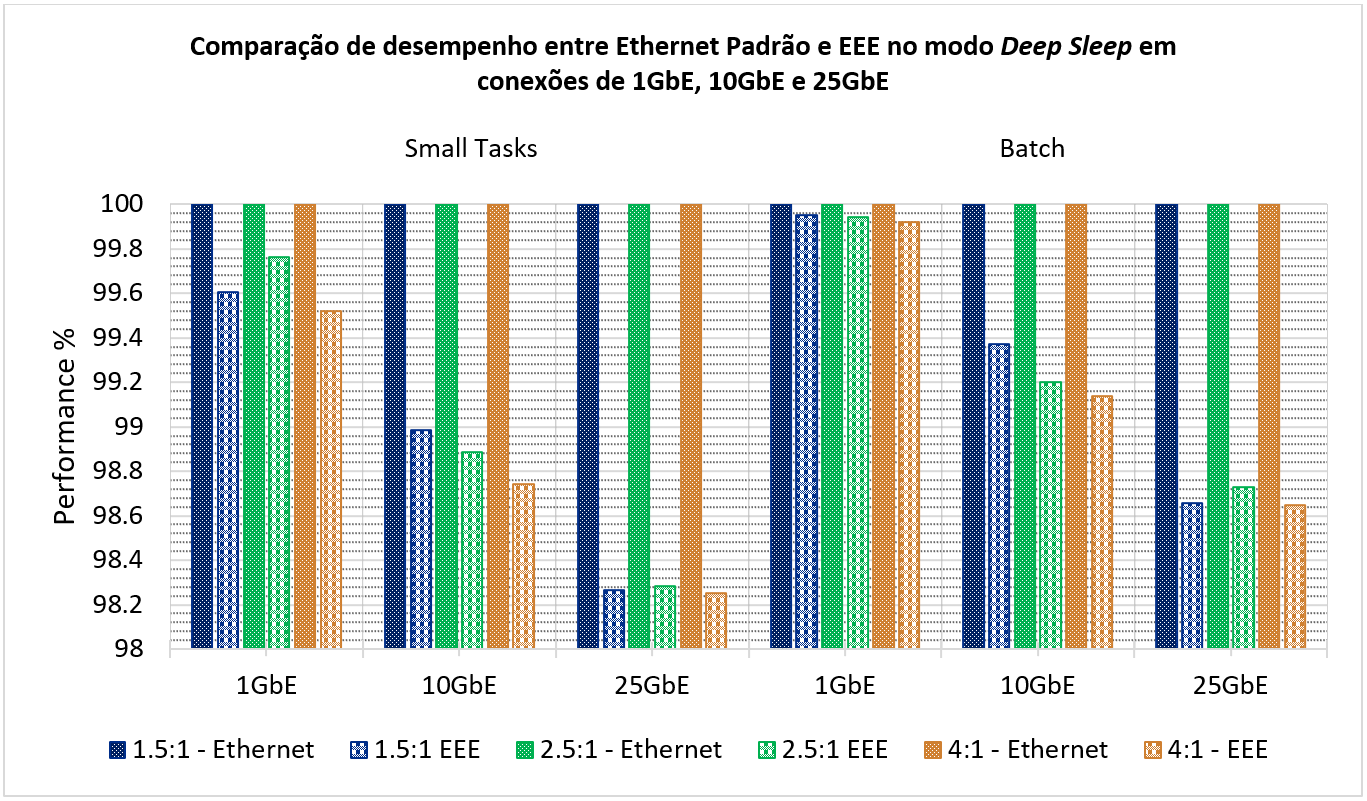
\includegraphics[width=16cm]{4-EEEHadoop/Image3_EEEPerformance1-10-25.PNG}
    \caption{\centering Comparação de desempenho entre \emph{Ethernet} Padrão e EEE no modo \emph{Deep Sleep} em conexões de 1GbE, 10GbE e 25GbE}
    \label{fig:EEEPerformance1-10-25}
\end{figure}

\begin{figure}[htp]
    \centering
    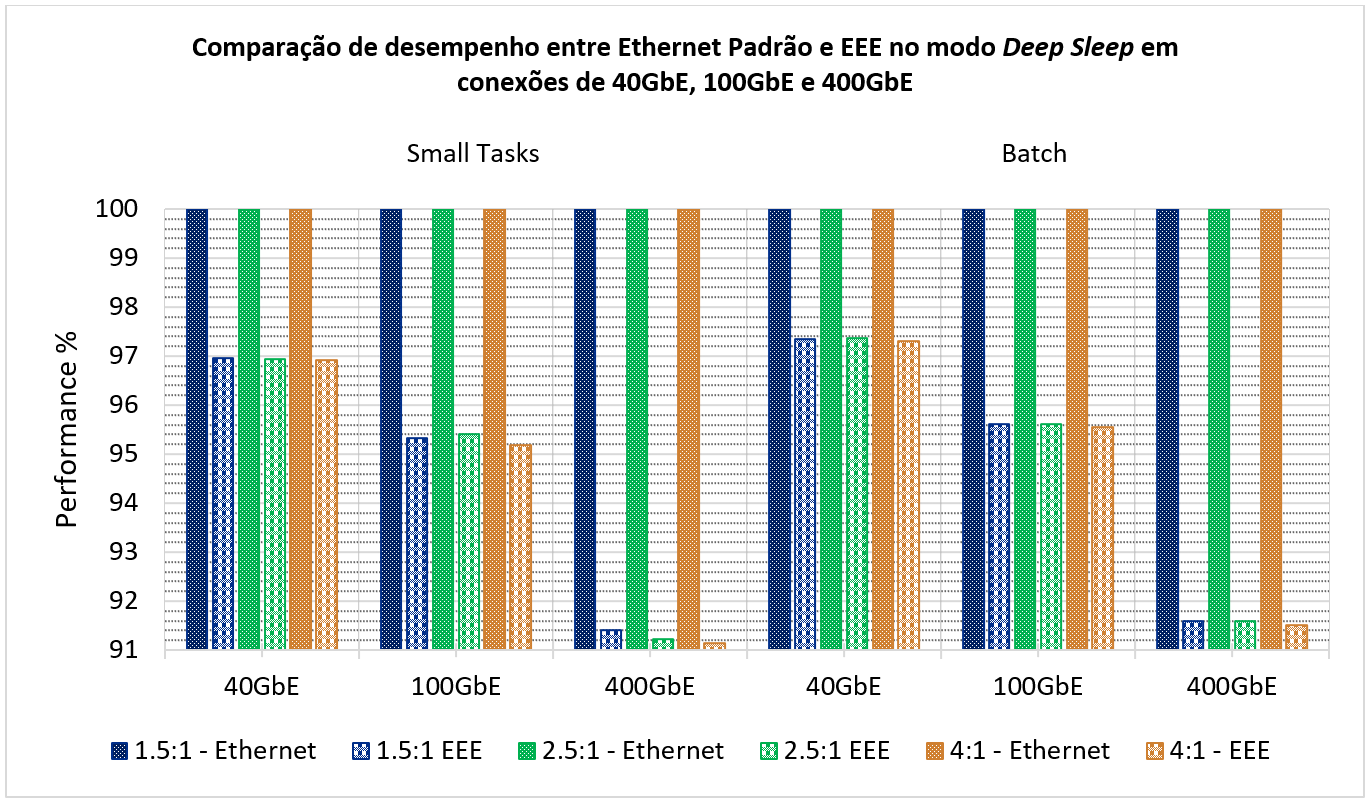
\includegraphics[width=16cm]{4-EEEHadoop/Image4_EEEPerformance40-100-400.PNG}
    \caption{\centering Comparação de desempenho entre \emph{Ethernet} Padrão e EEE no modo \emph{Deep Sleep} em conexões de 40GbE, 100GbE e 400GbE}
    \label{fig:EEEPerformance40-100-400}
\end{figure}

\begin{figure}[htp]
    \centering
    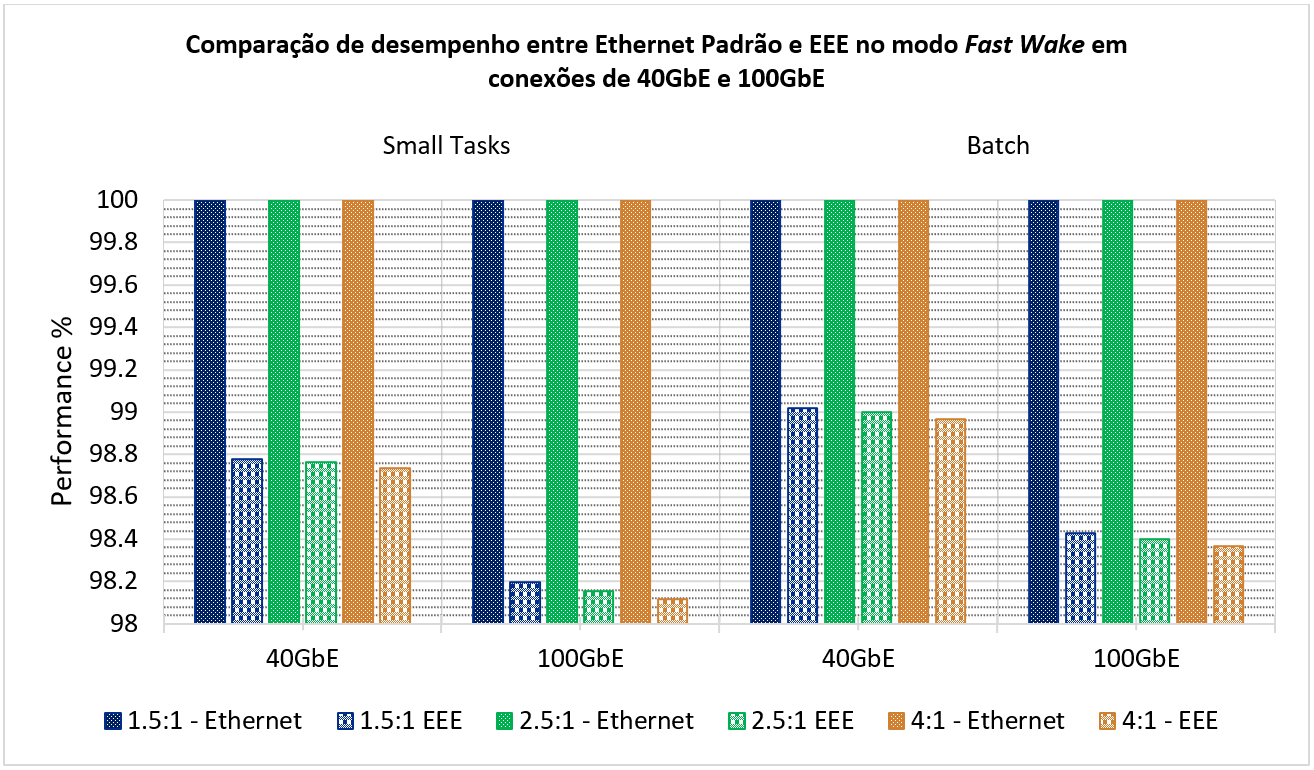
\includegraphics[width=16cm]{4-EEEHadoop/Image6_EEEPerformance40-100-FastWakeMode.PNG}
    \caption{\centering Comparação de desempenho entre \emph{Ethernet} Padrão e EEE no modo \emph{Fast Wake} em conexões de 40GbE e 100GbE}
    \label{fig:EEEPerformance40-100FastWake}
\end{figure}

Ao utilizarmos o modo \textbf{\emph{Fast Wake}} do EEE em nossas simulações, foi possível notar que embora este modo não forneça uma economia de energia como o modo \textbf{\emph{Deep Sleep}}, ele não afeta o desempenho de forma que seja considerável, com uma perda de 1,2\% no caso das conexões de 40GbE e 1,8\% em conexões de 100GbE, tornando-se assim uma opção interessante para as indústrias que buscam um balanceamento entre economia de energia e desempenho.  

As perdas de desempenho mais significativas encontradas para os links de 100GbE e 400GbE com o modo \textbf{\emph{Deep Sleep}} ocorreram porque em determinados momentos é necessário acordar um link para transmitir um único \emph{frame}, o que causa penalidades de latência e consumo de energia em termos relativos que são agravadas de acordo com a largura de banda \cite{jiang2021modeling}; \cite{reviriego2009performance}; \cite{reviriego2010burst}; \cite{e2017energy}. Se os momentos de \emph{wake} do EEE puderem ser controlados para evitar transmissões de um \emph{frame} único, pode ser possível obter economia de energia com perdas de desempenho baixas ou nulas para estas conexões.

\section{Considerações Finais}

Neste capítulo, apresentamos uma análise do impacto ao habilitar ao \emph{Energy Efficient Ethernet} nos modos \textbf{\emph{Deep Sleep}} e \textbf{\emph{Fast Wake}} em \emph{clusters MapReduce} que utilizam o \emph{framework} Apache Hadoop 3.x. Avaliamos execuções de \emph{Small Tasks} e \emph{Batch Jobs} com EEE em diversos \emph{clusters} simulados, e no modo \textbf{\emph{Deep Sleep}} encontramos economia de energia entre 78\% e 82\% para links de até 40GbE sem perda considerável de desempenho, entre 0,21\% e 2,85 \%. Para links de 100GbE e 400GbE houve uma economia de energia significativa de 75,69\% e 51,88\% respectivamente, mas com uma taxa de perda de desempenho considerável de 4,55\% e 8,58\%, o que não é particularmente interessante em \emph{Batch Jobs}. Quando optamos pelo uso do modo \textbf{\emph{Fast Wake}} do EEE, obtivemos uma redução do consumo de 7,49w/h para 4,634w/h em conexões de 40GbE, e de 10,89w/h para 6,916w/h em conexões de 100GbE, com uma perda de performance de 1.2\% e 1.8\%.

Em termos de custo-benefício para \emph{data centers}, o recomendado para conexões de até 40GbE é habilitar o EEE no modo \textbf{\emph{Deep Sleep}}, o que resulta em uma boa redução do consumo de energia e uma taxa de perda de desempenho baixa ou nula. Para conexões de 100GbE o recomendado é habilitar o modo \textbf{\emph{Fast Wake}} do EEE, obtendo assim um balanceamento entre consumo de energia e performance. Para conexões de 400GbE habilitar o EEE não é interessante, pois há uma perda de 8,58\% do desempenho.

O problema de latência e economia de energia encontrado em conexões acima de 100GbE com \textbf{\emph{Deep Sleep}} são causados por ter que acordar o link de tempos em tempos para transmitir um único \emph{frame}. Para resolver este problema, no próximo capítulo combinamos o \emph{Energy Efficient Ethernet} com \emph{Packet Coalescing}, \emph{Random Early Detection}, \emph{Controlled Delay}  e \emph{Explicit Congestion Notification}, podendo assim configurar de forma manual e inteligente quando os links devem ser acordados do modo LPI para transmissões de pacotes.

